% The preamble has been dumped out as out/presentationpreamble.fmt file. You can recreate that file by
% xelatex -ini -jobname="pinholepreamble" -output-directory=out "&xelatex pinholepreamble.tex\dump"
% 
% To compile you need to load that binary file using -fmt option
% xelatex -fmt out/pinholepreamble.fmt -output-directory=out pinhole.tex
%\documentclass[10pt, compress]{beamer}
\usetheme[usetitleprogressbar]{m}
 
 \usepackage{booktabs} % for better tables
 \usepackage{media9} % for includemedia i.e. videos
 \usepackage{xcolor} % for more colors
 \usepackage{hyperref} % for links
 \usepackage{cutwin} % text wrapped around figures
 \usepackage[backend=bibtex]{biblatex} % fancy citations
 
\usepackage{tikz}
\usetikzlibrary{shadows,trees}
\usetikzlibrary{shapes,calc,backgrounds}
\usepgfplotslibrary{dateplot}


%\tikzset{external/system call={xelatex -fmt out/pinholepreamble.fmt \tikzexternalcheckshellescape -shell-escape -halt-on-error -interaction=batchmode -jobname "\image" "\texsource"}}
%

% transparency
%\setbeamercovered{transparent=15}

\title{Pinhole camera}
\date{\today}
\author{Vikas Dhiman\\ David Johnson\\ Jason J Corso}
\institute{University of Michigan}
\bibliography{pinhole}

\begin{document}
\maketitle
\begin{frame}{Contents}
  % This slide will be removed later
  \tableofcontents
\end{frame}
% \begin{frame}{Sources}
%   \begin{itemize}
%     \item 
%       \url{http://www.exploratorium.edu/science_explorer/pringles_pinhole.html}
%     \item
%       \url{http://www.learner.org/workshops/sheddinglight/}
%   \end{itemize}
% \end{frame}
% \begin{frame}{Pinhole camera}
%   \centering
%   \includegraphics{media/girl_looks.png}
% \end{frame}

\section{About Light}
% Interesting notes/facts/videos about how human eye works.
% First camera "possibly" developed by ancient greeks and ancient Chinese.
% First documented description of a camera dates back to 1021 AD by a Arab physicist Ibn al-Haytham in his "Book of optics"
%%
%% How do you think our eyes work?
%% 
%% 
%% or 
%% 
%% 
% Rhetoric questions? Get kids involved
% What do kids think, how does eye/camera work?
\begin{frame}{How do you think our eyes work?}
  \begin{columns}
    \begin{column}{0.8\textwidth}
      \begin{itemize}
        \item
          Does the ``sight'' travel from our eyes to the object?\\
          \visible<2-> {\color{red}{Euclid other Greek believed so around 300 BC}\footfullcite{BBC:Let there be Light (2006)}}
        \item
          \color{black}{or the ``light'' travels from the object to our eyes?}\\
          \visible<3-> {\color{red}Modern scientists the believe so, and I have no reasons to question them.}
      \end{itemize}
    \end{column}
    \begin{column}{0.2\textwidth}
        \includegraphics[width=\columnwidth]{media/lghtmisc2.png}
    \end{column}
  \end{columns}
\end{frame}

% \begin{frame}{What does it mean to see things?}
% 
% \end{frame}

\begin{frame}{What is light?}
  \begin{columns}
    \begin{column}{0.7\textwidth}
      \begin{itemize}
        \item Greek philosophers believed that sight was possible because of interaction of fire in eyes and in the sun.
        \item Euclid, a Greek philosopher, gave  us some particular insights about light.
      \end{itemize}
    \end{column}
    \begin{column}{0.3\textwidth}
      \includegraphics[width=\columnwidth]{media/Euklid.jpg}
    \end{column}
  \end{columns}
\end{frame}

\begin{frame}{Light travels in straight lines}
  \footfullcite{BBC:Let there be Light (2006)}
    \includemedia[label=euclid-straight-lines,
      width=\linewidth,height=0.6\linewidth, % 16:9
      activate=pageopen,
      addresource=media/euclid-straight-lines.mp4,
      flashvars={
        source=media/euclid-straight-lines.mp4
        &loop=false             % loop video
        &scaleMode=letterbox   % preserve aspect ratio while scaling the video
      }
    ]{\includegraphics{media/euclid-straight-lines.png}}{VPlayer.swf}
\end{frame}

\section{Making a pinhole camera}
\frame{\tableofcontents[currentsection]}
\begin{frame}{Step 1}
  \begin{columns}
    \begin{column}{0.4\textwidth}
      Take the plastic lid off the Pringles® can and wipe out the inside. (Save the lid!)
    \end{column}
    \begin{column}{0.6\textwidth}
      \includegraphics{media/upside_down_vase.png}
    \end{column}
  \end{columns}
\end{frame}

\begin{frame}{Step 2}
  \begin{columns}
    \begin{column}{0.4\textwidth}
Draw a line with the marker all the way around the can, about 2 inches up from the bottom. Have a grown-up cut along that line so the tube is in two pieces.
    \end{column}
    \begin{column}{0.6\textwidth}
      \includegraphics{media/hand_pencil.png}
    \end{column}
  \end{columns}
\end{frame}

\begin{frame}{Step 3}
  \begin{columns}
    \begin{column}{0.6\textwidth}
      \begin{itemize}
        \item 
          The shorter bottom piece has a metal end. With the thumbtack, make a hole in the center of the metal.
        \item
          We're going to use the plastic lid as a screen. If your lid is clear, you may need to apply a piece of wax paper, white tissue paper, or vellum to the lid to act as a translucent screen. Put the plastic lid onto the shorter piece. Put the longer piece back on top. Tape all the pieces together.
      \end{itemize}
    \end{column}
    \begin{column}{0.4\textwidth}
      \includegraphics{media/can_cut_off.png}
    \end{column}
  \end{columns}
\end{frame}

\begin{frame}{Step 4}
  \begin{columns}
    \begin{column}{0.6\textwidth}
To keep light out of the tube, use a piece of aluminum foil that's about 1 foot long. Tape one end of the foil to the tube. Wrap the foil all the way around the tube twice, then tape the loose edge of the foil closed. If you have extra foil at the top, just tuck it neatly inside the tube.
    \end{column}
    \begin{column}{0.4\textwidth}
      \includegraphics{media/can_cover.png}
    \end{column}
  \end{columns}
\end{frame}

\begin{frame}{Pinhole camera is ready to use}
  \centering
  \includegraphics{media/girl_looks.png}
\end{frame}

\section{How does it works}
\begin{frame}{About light}

Learning Objectives

\begin{itemize}
  \item 
    Light energy travels in straight lines until it strikes a surface.
  \item 
    A shadow is formed when an object blocks the photons that are traveling from a light source.
  \item 
    Light travels fast, but not instantaneously.
  \item 
    We see because light from a source is reflected from an object to our eyes.
\end{itemize}
\end{frame}

\begin{frame}{Ray diagram}
  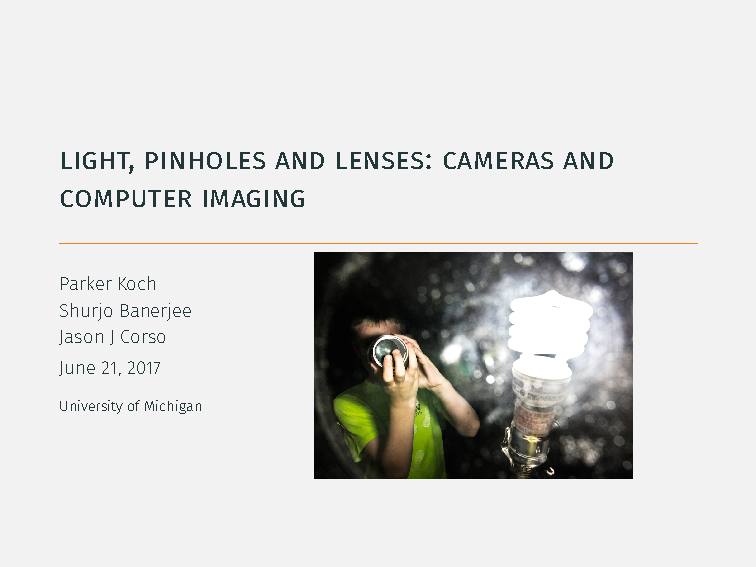
\includegraphics[width=\textwidth]{media/pinhole.png}
\end{frame}

\begin{frame}{Find the distance }
  Can you find the distance of the object given the size of object.
\end{frame}

\begin{frame}{Similar triangles}
  \includegraphics[width=\textwidth]{media/tri-similar1.png}
\end{frame}

\begin{frame}{Ray diagram}
  \includegraphics[width=\textwidth]{media/pinhole_blurred.png}
\end{frame}

\begin{frame}
  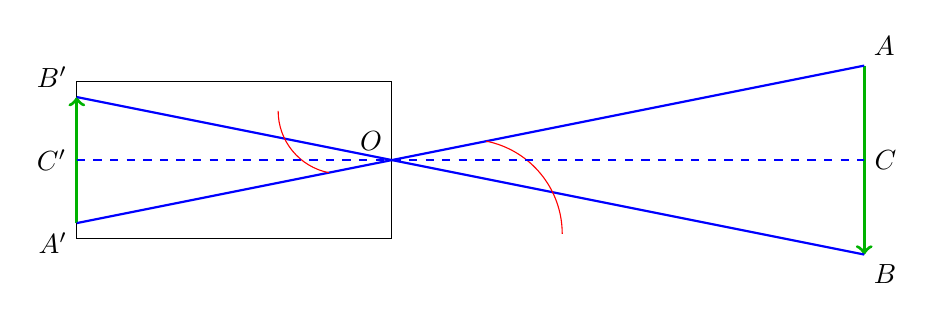
\begin{tikzpicture}
    \draw (-4,-1) rectangle (0, 1);
    \coordinate [label=above left:$O$] (origin) at (0,0);
    \coordinate [label=below left:$A'$] (imga) at (-4, -0.8);
    \coordinate [label=above left:$B'$] (imgb) at (-4, 0.8);
    \draw [->,very thick,green!70!black] (imga) -- (imgb);
    \coordinate [label=above right:$A$] (obja) at (6, 1.2);
    \coordinate [label=below right:$B$] (objb) at (6, -1.2);
    \draw [->,very thick,green!70!black] (obja) -- (objb);

    \draw [thick,blue] (imga) -- (obja);
    \draw [thick,blue] (imgb) -- (objb);
    
    \draw [red] let 
    \p1 = ($ 0.2*(imga) $),
    \n1 = {atan2(-\x1, -\y1)} 
    in (\x1,\y1) arc (\n1:0:\x1);

    \draw [red] let 
    \p1 = ($ 0.2*(obja) $),
    \n1 = {atan2(\x1, \y1)} 
    in (\x1,\y1) arc (\n1:0:\x1);

    \draw [thick,blue,dashed] ($0.5*(imga)+0.5*(imgb)$) node [text=black,anchor=east] {$C'$} -- ($0.5*(obja)+0.5*(objb)$) node [text=black,anchor=west] {$C$};
  \end{tikzpicture}
  \centering
  \begin{align}
    \frac{AC}{OC} = \frac{A'C'}{OC'}
  \end{align}
\end{frame}

\begin{frame}

  Can we compute the distance of object?
  
\end{frame}

\begin{frame}{Multiple pinholes}

  What happens when we make multiple pinholes?
  
\end{frame}

\begin{frame}{Bigger pinhole}

  What happens we make pinhole to a pencil-hole?
  
\end{frame}

\section{Introducing a lens}

\begin{frame}

  Now try using a lens?
  
\end{frame}

\begin{frame}{Iteractive animation}

  \url{http://www.pbslearningmedia.org/resource/lsps07.sci.phys.energy.geometoptics/geometric-optics/}

\end{frame}
\end{document}
